% !TEX root =  master.tex
\newcommand{\dutzi}{Prof. Dr. Dennis Dutzint\xspace}
% -------------------------------------------------------
% Dozent
%
% -------------------------------------------------------
\cvsect{\dutzi}
\begin{minipage}[t]{0.5\textwidth}
	\vspace{-3.6cm}
	\renewcommand{\arraystretch}{1.5}
	\begin{tabular}{l l}
		Name: & \dutzi \\
		Alter: & 45 \\
		Tätigkeit: & Professor für Wirtschaftsinformatik \\
		Skills: & 4/5 \hspace{-1cm} \begin{barchart}{5.0}
			\baritemNL{}{4}
		\end{barchart} \\
	\end{tabular}
\end{minipage}
\hfill
\begin{minipage}[t]{0.4\textwidth}
	\flushright
	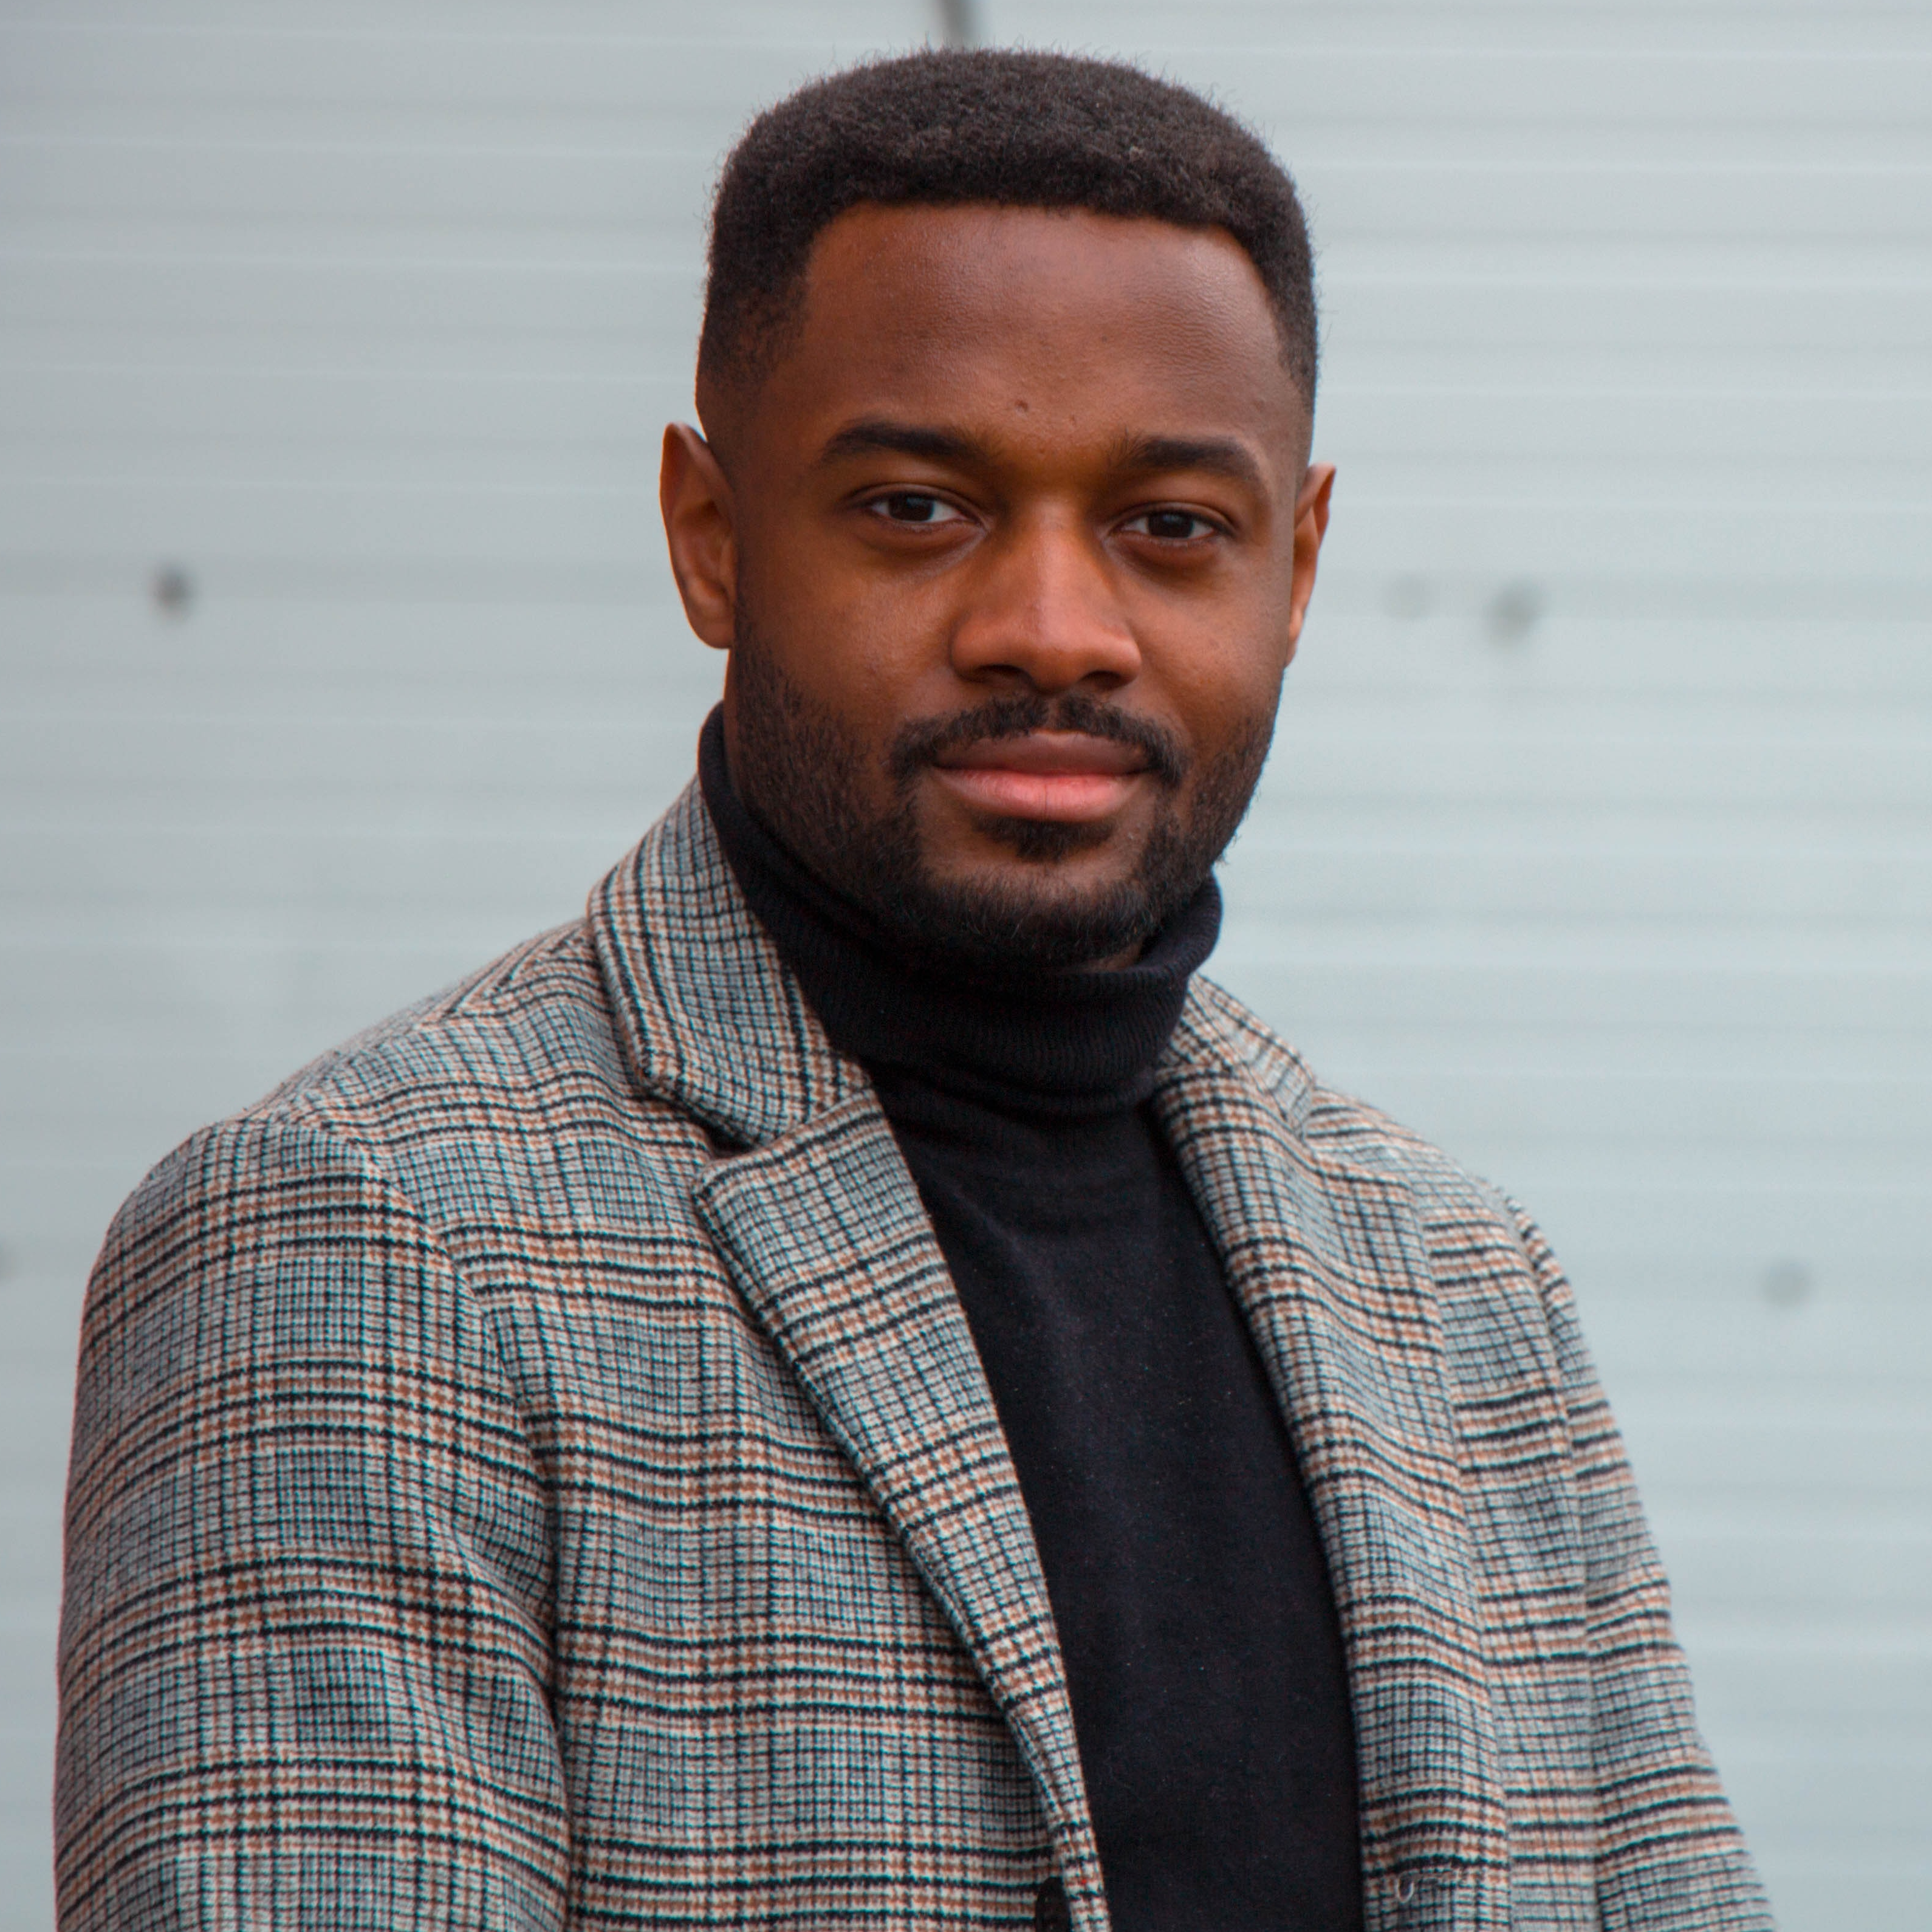
\includegraphics[width=0.70\textwidth]{img/personas/prof_dutzin2}
\end{minipage}
\autocite{rf-unsplash-dozent}

Das möchte ich gerne haben:
\begin{itemize}
	\item einfaches, schnelles und unkompliziertes Erstellen neuer Umfragen
	\item Auswertung von Umfrageergebnissen
    \item Wiederverwendung vorhandener Umfragen
    \item Verwaltung von Nutzern
\end{itemize}

Mit der ersten Persona, \dutzi, wird ein technikerfahrener Professor einer Hochschule beschrieben.
\dutzi nimmt primär die Rolle des Umfrageerstellers ein, wobei er für verschiedene Kurse unterschiedliche Umfragen erstellen und auswerten möchte.
Weiterhin möchte er die Rolle eines Administrators übernehmen und die Anwendung betreuen.
